\documentclass[12pt]{article} 
%\usepackage{bookman}
\usepackage{/home/weiliu/projects/haldefs}
\usepackage{graphicx}
\usepackage{url}
\usepackage{textcomp}
\usepackage{enumitem}
\usepackage{subfig}
\usepackage{hyperref}
%\usepackage{/home/sci/weiliu/packages/breakurl/breakurl}
\usepackage{amsmath}
\usepackage{verbatim}
\usepackage{fancyvrb}
\usepackage{natbib}
\usepackage{algorithmic}
\usepackage{algorithm}
\usepackage{color}
\usepackage{mdwlist}

\hypersetup{
  % bookmarks=true,         % show bookmarks bar?
    unicode=false,          % non-Latin characters in Acrobat’s bookmarks
    pdftoolbar=true,        % show Acrobat’s toolbar?
    pdfmenubar=true,        % show Acrobat’s menu?
    pdffitwindow=false,     % window fit to page when opened
    pdfstartview={FitH},    % fits the width of the page to the window
    pdftitle={Pulmonary Vessel Segmentation Notes},
    pdfauthor={Wei Liu},     % author
    pdfsubject={Reading notes},   % subject of the document
    pdfcreator={Wei Liu},   % creator of the document
    pdfproducer={Producer}, % producer of the document
    pdfkeywords={Pulmonary vessel, segmentation}, % list of keywords
    pdfnewwindow=true,      % links in new window
    colorlinks= true,       % false: boxed links; true: colored links
    linkcolor=blue,          % color of internal links
    citecolor=blue,        % color of links to bibliography
    filecolor=magenta,      % color of file links
    urlcolor=cyan           % color of external links
}


\setlength{\oddsidemargin}{0 in}
\setlength{\evensidemargin}{0 in}
\setlength{\topmargin}{-0.6 in}
\setlength{\textwidth}{6.5 in}
\setlength{\textheight}{9 in}
\setlength{\headsep}{0.5 in}
\setlength{\parindent}{0 in}
\setlength{\parskip}{0.1 in}



\begin{document}
\title{Pulmonary Vessel Segmentation Notes}
\author{Wei Liu}
\maketitle

The extraction and segmentation of lung vessels have two category: Region-based,
or appearance model, assign each voxel a label of vessel or non-vessel. The
path-based methods use geometrical features to track the vessel, and only
explore a sparse subset of the voxel space.

Here are a few options for automatic, or semi-automatic extraction of the lung vessels:

\begin{itemize}
  \item Machine learning methods. We can define features for each voxel, such as
    Hessian matrix features, and learn a classifier from the labeled data. The
    extraction of vessels in test image do not need user input of seed
    voxels. The feature may need careful selection.

  \item Minimal path methods, such as Dijkstra's algorithm explore the possible
    vascular trees given initial seed point. If a full automation of extraction
    is too difficult, Dijkstra's algorithm is able to find the vessel path from
    a single-source voxel. Existing works mostly use minimal path methods for
    tracking the centerline. But with a single source point, we can use such
    methods for exploring the whole space, and find those pixels that is
    connected to the source point via a path of costs below certain threshold.
    
  \item Particle-filter method, and Markov point process method. (to be added)
\end{itemize}

Since some labeled lung vessel images are available, one question is how to
use these information. For single-source tracking methods, the training data
can be used to define the source region. Because only the labels of the large
vessels are available, and only the large vessels can be assumed to be in the
same coordinates even after between-subject registration, we probably only use
these large vessels.

For ML-based method, the labeled images can be used to train a
classifier. Either minimal path methods or ML-based methods, we need good
features, or filters to detect the vessel structures.

Feb 10: My plan: 1) write multi-scale Frangi's Hessian vesselness feature
extractor. 2) Dijkstra's algorithm. 3) Explore the geodestic voting algorithm
of Mille and Cohen, 2009.

2/11: Study the Lemon graph library and found it has the Dijkstra's algorithm
for find the minimal path give a source node. the algorithm actually return a
accumulative cost map, and can easily find the path of each destination
node. Will use Lemon graph library in implementing the vessel extraction code.

A very promising extension of the shortest path methods is
\cite{rouchdy2011geodesic}, where the shortest path to multiple destination
points are accumulated to a path map, a high score in the path map indicates
larger probability of being vessel. the good thing of this method is relatively
easy of implementation, and the easy thresholding of the path map compared with
thresholding the cost map of the original Dijkstra's algorithm. But we shall
start from the basic Dijkstra method.

2/12: Implemented the vessel extraction code with Lemon. Build the vessel
project with cmake, build a directed graph from the input 3d volume. Need to
find a good way to define the cost of the arcs. We have the vesselness on each
voxel (nodes), but not on the arcs. A large vesselness on two adjacent nodes
means a small cost of current arc. From \cite{lesage2009review} I found
\cite{gulsun2008robust} which defines the cost of the edges by the directional
Hessian features. For now, we have only the vesselness value as a scalar value,
so it is not possible to do the same thing. But it make sense to have a
directional features, maybe in the future.

While the geodesic voting method has one source and multiple destinations, I
wonder if we can have multiple source and multiple destinations for more
robust results, and also not having to manually input the source
node. Together with the bidirectional path searching (see
\cite{lesage2009review} and the reference therein), the computation cost is
probably reasonable?

It seems \cite{olabarriaga2003minimum} got a lot reference from
\cite{wink2000minimum}. Need to study how these works use bidirectional
shortest-path method. Also check out the early freezing method mentioned in
\cite{lesage2009review}, for a possible speed-up of the searching.

1/13: Done with a very basic Dijkstra shortest path algorithm. According to
the Lemon graph document, the Dijkstra's algorithm of Lemon can define
multiple source nodes, and find the shortest path over the multiple source
nodes. This will be a possible feature we need to add. Actually we can choose
the same set of nodes as

Also need to study the parameters of the itk filter, $\alpha_1$ and
$\alpha_2$.

3/4: In order to constrain the computation within the lung, we need to segment
the lung from the rest of the body. It seems the artery has very similar
intensity with the body's wall, and it is difficult to find a good threshold
to differentiate them apart. However, we can probably segment the lung
out, and use the surface of the lung to define the destination  points for
minimal-path searching. 

The gray level intensity have 5 components:
\begin{itemize}
\item component 1, with mode -1000. Mostly are background and body wall.
\item Component 2, with mode -800, mostly are lung.
\item Component 3, with mode -100, body wall.
\item Component 4, with mode 50, mostly body wall and tissues of no interest. 
\item Comp 5, with mode 560, vein. The intensity of the vein is larger than
  the arteries, probably because the injected  dye go through the vein first
  with higher concentration. 
\end{itemize}

Among the 5 components, component 4 and 5 are difficult to differentiate. The
voxel intensity between the modes of the two components includes arteries and
the un-interesting tissues. 

We need to run a Gaussian mixture model with 5 Gaussian components. The
initial component centers will be hard-coded to the above empirical
value. Once we estimate the label of each pixel, we can remove specific
components to get the set of pixels in the lung. Also, the likelihood of the
pixel being in certain components are used in the cost definition of the
minimal-path method. 

3/8: Got the first results on real lung CT data. Use the full body mask to
choose pixels within the body, and use the lung mask to choose destination
points on the lung surface. Showed the path from the starting point to a
single target point, and found the path wiggles. May need a regularization
on the total length of the path, besides minimizing the total sum of
cost. Refer to Cohen's paper. 

3/14: My version of multiscale Hessian works now. By running the filter on a
toy example, I found the detected optimal sale is 1/3 of the size of the
original object.

A test on the toy data (lines) shows that the vesselness looks better when I
choose to scale the vesselness by the magnitude of the largest absolute
eigenvalue.

3/17: A test on the real data (PE105) shows that scaling the vesselness seems
to remove the false-positive structures. Also show the 3D volume in Slicer. So
for now, I will use the scaled version of the multiscale Hessian filter. The
output vesselness is not in (0, 1) anymore due to the scaling. Have to find a
way to re-normalize it to (0, 1). 

On the PE105 data, both the scaled and non-scaled vesselness image have big
value inside of the heart. Such big vesselness values do not make sense,
because the heart should not have large Frangi vesselness value. The scaled
vesselness have value around 200 inside the heart. Such value is even bigger
than many true vessels. For non-scaled volume, the value inside the heart
reaches 0.6, 

My version of multiscale Hessian filter takes too much memory. Need to change
all double precision data structures to single. 

\begin{figure}[htb]
  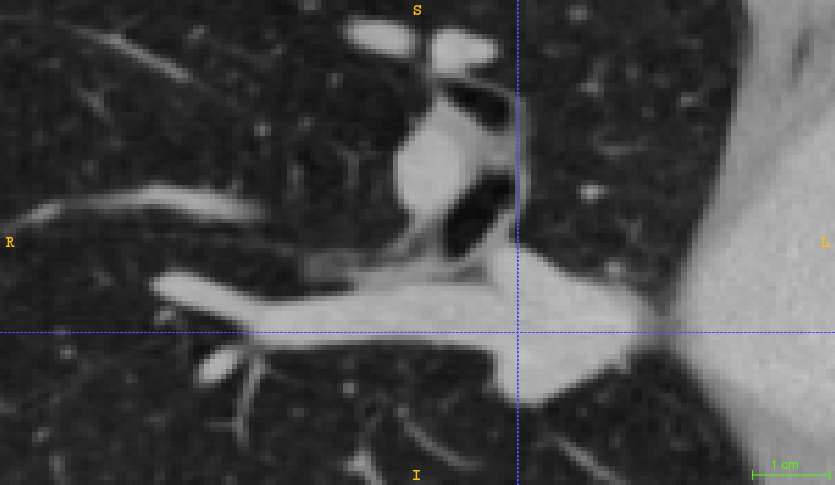
\includegraphics[width=0.3\textwidth]{figures/vesselness/cta}
  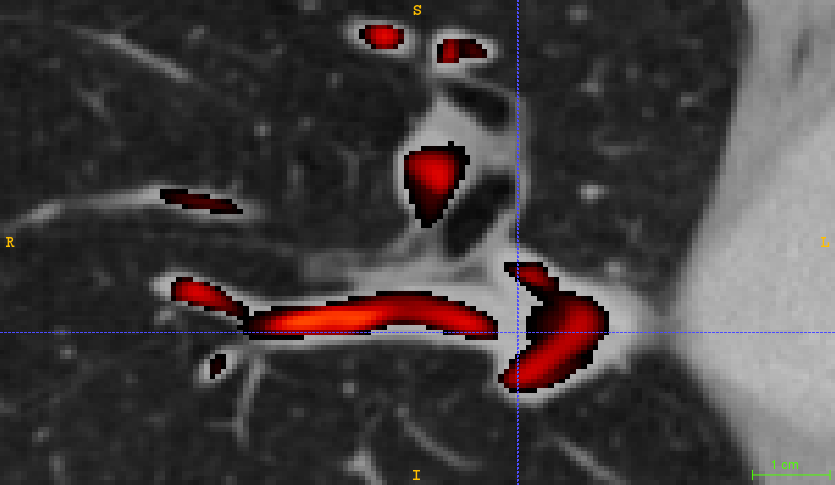
\includegraphics[width=0.3\textwidth]{figures/vesselness/vesselness}
  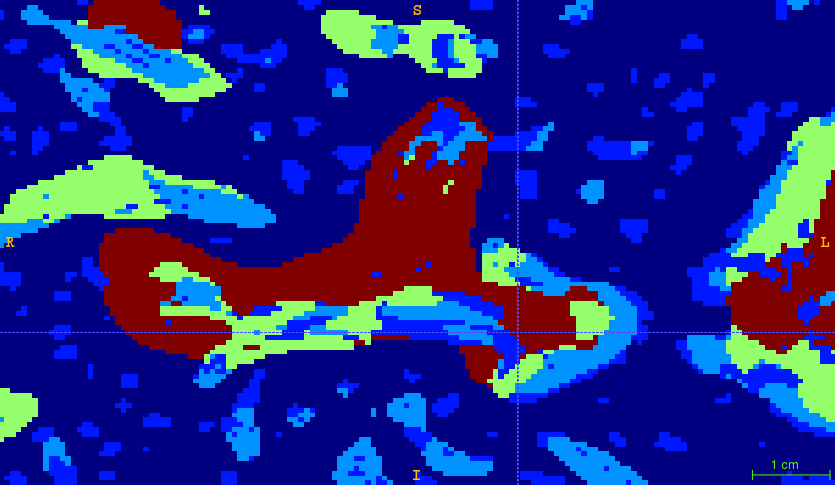
\includegraphics[width=0.3\textwidth]{figures/vesselness/scale}\\
  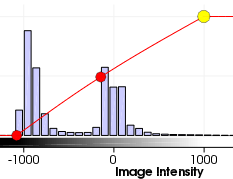
\includegraphics[width=0.3\textwidth]{figures/vesselness/cta_colormap}
  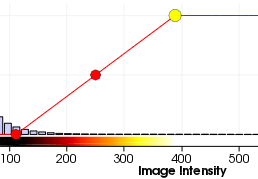
\includegraphics[width=0.3\textwidth]{figures/vesselness/vesselness_colormap}
  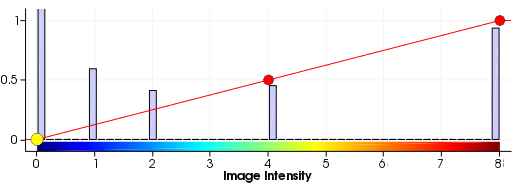
\includegraphics[width=0.3\textwidth]{figures/vesselness/scale_colormap}
  \caption{The vesselness and optimal scale map of pulmonary vessels. Left:
    the original CTA image. Middle: vesselness map, with values below certain
    values not shown. Right: optimal scale, rendered in color. The vesselness
    measure of the horizontal vessel structure is broken in the middle,
    because the interference of other structures. From the scale map,
    Vesselness detector believes the middle part is a larger structure, hence
    the scale map has larger value in the middle. }
\end{figure}

3/20: Vesselness need to be normalized before use. The test on the ``line''
data shows that when vessleness value in the range of (0, 0.1), the Dijkstra
method cannot find the correct cost map. Multiplying the original vesselness
value by a large number 1000 will solve the issue. In practice, we may need to
normalize the vesselness using it's maximum value (or a robust maximum value
after removing the outliers). Check out ITK's function for the quantile. 

ITK has histogram filter that can compute the percentile, and we can use it to
remove the extremely big value from the vesselness map, since this is not the
portion that we are interested in. The vesselness map will be saturated at
certain percentile, for example, 99 percentile. We do not need threshold lower
range since a large portion of the vesselness map will be zero.

3/21: The large vessels may not look like tube structure, so the Frangi's
vesselness measure may fail. It make sense to start with one or more seeds,
and use level-set method to extract those large vessel regions. After that, we
can use Frangi's vesselness measure and also Hessian matrix eigenvector for
guiding the extraction of the small vessel structures. It would be good to
have a framework that I can combine the two method together. Need check out
the review paper. I remember there are some works that use vesselness features
to guide the more standard segmentation approach, such as region growing, or
level-sets methods. 

3/24: Test on the PE105 dataset. Choose a point in the heart region with large
vesselness value. When debugging into the code, found the unscaled vesselness
is 0.5. But after scaling by the largest eigenvalue (321), the vesselness
value is much larger (185). So, the large eigenvalue is the reason of this
false-positive.

A few example coordinates of interest:

(230, 239, 134): The heart region where the vesselness gives the
false-positive results. Largest $lambda$= 321. The false-positive is due to
the too large $lambda$, and we choose to scale the Frangi's vesselness by the
largest eigenvalue. So, even the original vesselness is small, after
multiplying a large eigenvalue, the final vesselness measure 185) is incorrectly
large. 

(165, 318, 146): A true positive vessel. Without scaling, vesselness is
0.79. After scaling by $\lambda = 204$, the final vesselness is 161. So the
previous false-positive pixel has a vesselness value similar to this
true-positive, which is incorrect. 

(153, 297, 146): a non-vessel pixel. Before scaling, vesselness is 0.72, but
after scaling, the vesselness is 12.42. This is because the largest eigenvalue (17)
is small at this point. 

So we need the scaling of $\lambda$ take effect at 17, but not in the range of
(204, 321). Instead of scaling by $\lambda$, we should scale by $\log
\lambda$. As a result, at small values, $\log \lambda$ approximate a linear
function, hence having effect on scaling. At large value range (204, 321)
$\log$ function will make the difference of 204 and 321 much less than their
linear difference.

Comparing the true-positive pixel and false-positive, we found the
false-positive pixel has smaller value of $R_A$ of the Frangi vesselness
equation. Therefore, one possible way of having less false-positive is set a
larger value of $\alpha$, so the pixel with smaller $R_A$ will have smaller
vesselness value.

On the other hand, changing $\beta$ should not work, since the false-positive
pixel has even smaller value of $R_B$ than the true-positive. In another word,
the false-positive even looks more like vessel if measured by $R_B$.

Another issue is the vesselness measure tends to fail at the large vessel
structures. We should somehow combine the vesselness and the gradient
information to define a new speed map used for fast marching method. The speed
map will trust more the gradient (or the intensity) at larger vessels, and
trust the vesselness measures on smaller vessels. We can also use the scale
map to get a sense of the scale of the vessels for defining the speed map. For
example, if a pixel has a large optimal scale value on the scale map, we
assume the vesselness is less reliable than the gradient or intensity
information. One issue is, the scale map is not continuous, so we should
somehow have a smooth scale map for defining the speed map.

3/27: Have implemented the fast marching filter of ITK but not clear about the
stop criterion. The standard FM filter only can set values (i.e. the marching
time) for stop rule, but the Wiki page seems to say the base filter can set
volume size as a stop rule. After checking the source code (both v4.5 and
git), the only way of setting stop rule for both standard and base version is
the marching time value. I'm OK with that.

The base filter should be used only for the extension filter (with an extended
velocity filed), and the upwind filter (to compute the gradient at each pixel,
maybe useful for the voting method). For standard FM filter, we do not need
the base version. So, the term base is not for the standard FM filter. It was
confusing!

But even I understand that, I still don't know why the stop criteria are not
there.

Found the FM filter has leakage (similar to the leakage of region-growing
method). So, I need to tune the sigmoid filter such that the pixels at the
boundary have very small speed. 

After experimenting with the ITK FM method, and ITK-SNAP's level-set method, I
found it is difficult to extract the large vessels without leakage. Sometimes,
the artery leaks into the vein. So, the next step is to use the segmentation
of the training dataset as an starting seed regions, and run either ITK's fast
marching method, or my in-house version of the Dijkstra's method for
extracting the centerline. 

Or, we can combine the gradient magnitude map with the Frangi's vesselness map
to get a single speed map for FM method. The speed map will be in the form of
$\alpha G + (1-\alpha) V$, where $\alpha$ may depend on the scale map of the
multiscale Hessian filter.

3/28: A study of the ITK Fast Marching code seems to show that the base
version is newer, after the refactoring work of ITK. The base version depends
on ITK FM traits, so it should be relatively new. Will use the base version.

4/7: If I use the seed region's intensity as a reference, and compute a
probabilistic density map of each pixel being in the Gaussian distribution
defined by the seed region, we can get good results on the fast marching. 

The artery and vein may have different distribution with regard to the seed
region, i.e., the bias. Need look into that. 

4/8: Difference method to choose ending points for voting: we can run FFM
sufficiently long time, so the front end reaches out enough distance, but
probably still not reach the surface of the lung. Then using all the points on
the front end as the ending point for voting. 

4/14: It is impossible to use a GUI program in the Visceral virtual machine,
even I installed X11 server on the VM. Got error ``X11 forwarding request
failed'' error when logging in.

4/23: In this week, I will explore the image registration method. We need a
method that can build an atlas by using the data of multiple subject. Once we
have an atlas, we can add anatomical labels the atlas manually. This manual
labeling only need to be done once, and the labels will be mapped back to each
subjects.

The question to ask is, whether the current naive method of extracting vessels
is good enough for a statistical analysis of the vessel structure. 

4/24: Implemented a simple routine with simple ITK to compute the speed map by
the Gaussian density. Next step will be using fast marching to compute the
distance map with this speed map. 

\section{Vessel Extraction Pipeline}
5/7: Now trying to get a couple of subjects with lung, bone, and vessel
extracted. 

\begin{itemize}
\item Threshold the CT image at -2000 to get a \emph{cylinder} mask. The -2000
  value may change across patients?

\begin{Verbatim}[frame=single]
fslmaths /scratch/datasets/PE/PE000919.nii.gz -add 2000 -thr 0 -bin
PE919/round_mask.nii.gz
\end{Verbatim}


\item First run GMM with 3 components: lung, tissue, and bones. Initial
mean set to -800, 0, 1000, and initial standard deviation of GMM set to 100
for all components.  In some cases, we need to run GMM with 2 components.
\item Extract the components corresponding to th lung.
\begin{Verbatim}[frame=single]
sitkfuncs.extract_comp('RV01/RV01.nii.gz', 
'RV01/gmm_seg.nii.gz', 'RV01/cc.nii.gz')
\end{Verbatim}
\item Use ITK-SNAP to check the label corresponding to the lung. Mostly left
  and right lung are connected in a single component, so we need only one
  label. In rare case, they are separated into two components, so we need 2
  labels. 

\item Extract the lung component.

\begin{Verbatim}[frame=single]
 sitkfuncs.extract_lung('RV01/cc.nii.gz', [1], 
'RV01/lung.nii.gz', 10)
\end{Verbatim}

\item fill hole in the lung mask with the fillhole filter.

\begin{Verbatim}[frame=single]
fillhole_filter -i lung.nii.gz -o lung.nii.gz
\end{Verbatim}

\item Manually define seed regions.

\item Estimate the density and get a density map, which will be used as the
  speed map of fast marching method. 
\begin{Verbatim}[frame=single]
est_density -i RV01.nii.gz -e seeds.nii.gz -m lung.nii.gz 
-o density.nii.gz
\end{Verbatim}
  The standard deviation parameter of the density estimation routine controls
  how much belief the user should give to the seed region. With a small
  deviation, only the voxels with intensity close to the mean intensity of the
  seed regions will have larger density value. With a larger standard
  deviation, the voxel have non-zero density value even its intensity is quite
  different from the mean intensity. Therefore, the standard deviation
  parameter can be seen as a regularization. A larger value will make the
  density map more flat. Vessel and non-vessel voxels density will be similar,
  and fast marching have more chance to propagate to non-vessel regions.

  \item Run the fast marching method:
\begin{Verbatim}[frame=single]
fmm_upwind -p density.nii.gz -e seeds.nii.gz -m lung.nii.gz -t 500 
-o fmm_out.nii.gz
\end{Verbatim}

\item Inverse the value of the \emph{time of visit} map to get a heat map,
  where larger values represent vessels. 
\begin{Verbatim}[frame=single]
inverse_distmap -i fmm_out.nii.gz -m lung.nii.gz 
-o vessel.nii.gz -x 500
\end{Verbatim}
\end{itemize}

5/14: Trying to register two CT volume image using ANTS tool, with masks on
both fixed and moving images: 
\begin{Verbatim}[frame=single]
/scratch/packages/antsbin/bin/antsRegistration 
-d 3 
-o [PE000000_warp.nii.gz] 
-m MI[PE000105.nii.gz, PE000000.nii.gz, 1, 32] 
-t syN[0.01,0.1,1] 
-c 10x10x10 -s 3x3x3 
-f  4x2x1 
-x [PE000105.nii.gz, PE000000_mask.nii.gz]
\end{Verbatim}

The tool complains ``Too many samples map outside of image buffer''.

The, extract a small ROI of the PE105 as fixed image, and PE000 as moving
image:
\begin{Verbatim}[frame=single]
fslroi PE000000.nii.gz moving.nii.gz 138 200 165 150 184 102 
fslroi PE000105.nii.gz fixed.nii.gz 212 200 188 100 168 100 
\end{Verbatim}

And run antsRegistration without mask:
\begin{Verbatim}[frame=single]
/scratch/packages/antsbin/bin/antsRegistration -d 3 -o [xform,
moving_warpped.nii.gz] -m MI[fixed.nii.gz, moving.nii.gz, 1, 32]
-t syN[0.25,0.1,1] -c 10x10x10 -s 3x3x3 -f  4x2x1 
\end{Verbatim}

The registration process seems runs OK, but there is no affine transformation
output. The only output is the deformation matrix, and optionally the warped
moving images, which looks not good. 

6/12: ShapeWorks. Mayavi2 author's solution does not work. airway inspector
slow and no display screen. Got the Lynn PDF files. And studying the meshlab. 

Need to compare ShapeWorks and Spharm-pdm. 

Meshlab build no success, even commented out some filters. Asked James
Fishbaul and wait for response. 

6/13: build ShapeWorks with minimal options, success. With ``View'' option on,
fail. Asked Parasanna and the mail list and wait for the response. 

Spharm seems use the mesh to define the surface. 

6/16: Reading Josh Cates thesis, Spharm is a parametric method, and ShapeWorks
is non-parametric. Spharm only resprsent surfaces with spherical topologies. 

6/17: Add PowerCurst source code downloaded online into VTK5, but failed to
compile even commenting out some lines. 

Add PowerCrust source from Prasanna to ShapeWorks, and success to build after
commenting out erand48 related lines. Have a new option on the View2 panel. 

6/18: If we use CCA instead of PCA on a point distribution model, we can use
the class information during projection, such that the projection direction
maximize the difference between two groups.

 \bibliographystyle{plainnat}
\bibliography{/home/weiliu/projects/myref}
\end{document}
